\documentclass[11pt]{article}
\usepackage{amsmath, amssymb}
\usepackage[margin=1in]{geometry}
\usepackage{enumitem}
\usepackage{booktabs}
\usepackage{tikz}
\usetikzlibrary{arrows.meta, positioning, decorations.pathreplacing}

\title{U-Net Architecture and DDPM Practical Mechanics}
\author{Discussion Notes}
\date{March 2026}

\newcommand{\xb}{\mathbf{x}}
\newcommand{\eb}{\boldsymbol{\epsilon}}
\newcommand{\Ib}{\mathbf{I}}
\newcommand{\R}{\mathbb{R}}
\newcommand{\E}{\mathbb{E}}
\newcommand{\alphabar}{\bar{\alpha}}

\begin{document}
\maketitle

\noindent
This document describes the \emph{architecture and practical mechanics} of U-Nets
and DDPM. It complements \texttt{diffusion\_models\_introduction.tex}, which covers
the mathematical theory (forward/reverse processes, score functions, guided generation).
Here we focus on what each component does, how the pieces fit together, and the
specific choices for our 64$\times$64 grayscale image setting.

% ============================================================
\section{The U-Net Architecture}

\subsection{Why a U-Net?}

The score network $\eb_\theta(\xb_t, t)$ must take a noisy image and output a
tensor of the same spatial dimensions (the predicted noise). This input-to-same-size
mapping suggests an encoder-decoder structure. But a plain encoder-decoder
bottleneck discards spatial detail during compression---exactly the fine-grained
structure (edges, textures) that distinguishes natural images from noise.

A \textbf{U-Net} solves this with \textbf{skip connections}: direct pathways
from encoder layers to the corresponding decoder layers at the same spatial
resolution. The encoder extracts features at multiple scales; the decoder
reconstructs the output using both the bottleneck representation (global context)
and the skip connections (local detail).

\begin{center}
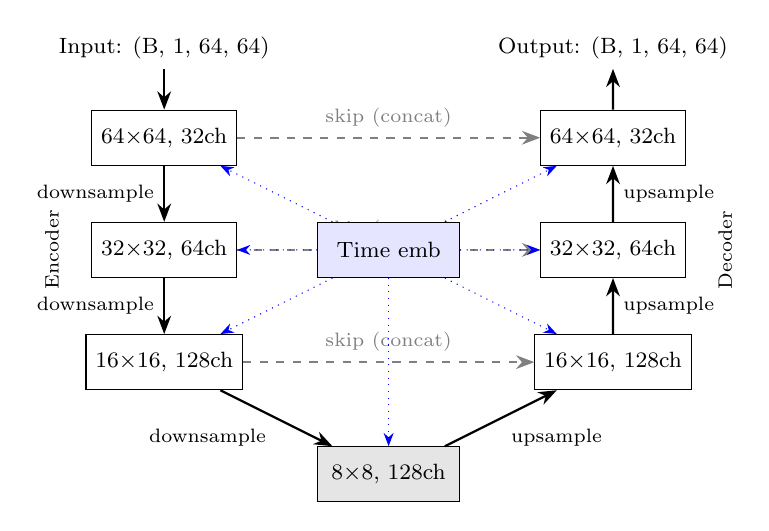
\begin{tikzpicture}[
    block/.style={rectangle, draw, minimum width=1.8cm, minimum height=0.7cm,
                  font=\footnotesize},
    skip/.style={-{Stealth}, dashed, gray, thick},
    flow/.style={-{Stealth}, thick},
    scale=0.95
]
% Encoder
\node[block] (e1) at (0, 0) {64$\times$64, 32ch};
\node[block] (e2) at (0, -1.5) {32$\times$32, 64ch};
\node[block] (e3) at (0, -3.0) {16$\times$16, 128ch};

% Bottleneck
\node[block, fill=gray!20] (mid) at (3, -4.5) {8$\times$8, 128ch};

% Decoder
\node[block] (d3) at (6, -3.0) {16$\times$16, 128ch};
\node[block] (d2) at (6, -1.5) {32$\times$32, 64ch};
\node[block] (d1) at (6, 0) {64$\times$64, 32ch};

% Input/Output
\node[font=\footnotesize] (inp) at (0, 1.2) {Input: (B, 1, 64, 64)};
\node[font=\footnotesize] (out) at (6, 1.2) {Output: (B, 1, 64, 64)};

% Encoder flow
\draw[flow] (inp) -- (e1);
\draw[flow] (e1) -- node[left, font=\scriptsize] {downsample} (e2);
\draw[flow] (e2) -- node[left, font=\scriptsize] {downsample} (e3);
\draw[flow] (e3) -- node[below left, font=\scriptsize] {downsample} (mid);

% Decoder flow
\draw[flow] (mid) -- node[below right, font=\scriptsize] {upsample} (d3);
\draw[flow] (d3) -- node[right, font=\scriptsize] {upsample} (d2);
\draw[flow] (d2) -- node[right, font=\scriptsize] {upsample} (d1);
\draw[flow] (d1) -- (out);

% Skip connections
\draw[skip] (e3.east) -- node[above, font=\scriptsize] {skip (concat)} (d3.west);
\draw[skip] (e2.east) -- node[above, font=\scriptsize] {skip (concat)} (d2.west);
\draw[skip] (e1.east) -- node[above, font=\scriptsize] {skip (concat)} (d1.west);

% Time embedding arrow
\node[block, fill=blue!10] (temb) at (3, -1.5) {Time emb};
\draw[-{Stealth}, blue, dotted] (temb) -- (e1);
\draw[-{Stealth}, blue, dotted] (temb) -- (e2);
\draw[-{Stealth}, blue, dotted] (temb) -- (e3);
\draw[-{Stealth}, blue, dotted] (temb) -- (mid);
\draw[-{Stealth}, blue, dotted] (temb) -- (d3);
\draw[-{Stealth}, blue, dotted] (temb) -- (d2);
\draw[-{Stealth}, blue, dotted] (temb) -- (d1);

% Labels
\node[font=\scriptsize, rotate=90] at (-1.5, -1.5) {Encoder};
\node[font=\scriptsize, rotate=90] at (7.5, -1.5) {Decoder};
\end{tikzpicture}
\end{center}

\subsection{Building Blocks}

Each encoder and decoder block consists of standard convolutional layers:

\paragraph{Convolutional block.}
Two consecutive operations: Conv2d $\to$ GroupNorm $\to$ SiLU activation.
The convolutions use $3\times3$ kernels with padding=1, which preserves spatial
dimensions. GroupNorm (instead of BatchNorm) is standard in diffusion models
because it is independent of batch size, which matters when using small batches
or single-image inference during sampling.

\paragraph{Downsampling (encoder).}
After each encoder block, spatial dimensions are halved. This is typically done
with a $4\times4$ convolution with stride~2 and padding~1, or equivalently a
$2\times$ average/max pooling followed by a $1\times1$ convolution. The stride-2
convolution is slightly more expressive (learnable downsampling) and is the
standard choice.

\paragraph{Upsampling (decoder).}
Spatial dimensions are doubled. Two standard approaches:
\begin{itemize}[nosep]
    \item Nearest-neighbor interpolation ($\times2$) followed by a $3\times3$ convolution.
          Avoids checkerboard artifacts from transposed convolutions.
    \item Transposed convolution (ConvTranspose2d) with stride~2.
\end{itemize}
We use nearest-neighbor + convolution for cleaner outputs.

\paragraph{Skip connections.}
At each resolution level, the encoder output is concatenated (along the channel
axis) with the decoder input at the same spatial resolution. If the encoder
produces $C$ channels and the decoder expects $C$ channels, the concatenation
produces $2C$ channels, which is then projected back to $C$ by the first
convolution in the decoder block.

This is the key mechanism: the decoder sees both the ``what is there'' (skip)
and the ``what should be there'' (upsampled bottleneck). For denoising, the skip
carries the noisy input features while the bottleneck carries the denoised
global structure.

\subsection{Time Conditioning}

The network must behave differently at different noise levels $t$. At high $t$
(heavy noise), it should predict the dominant noise structure. At low $t$
(light noise), it should predict subtle residual noise while preserving fine detail.

\paragraph{Sinusoidal embedding.}
The scalar timestep $t \in \{1, \ldots, T\}$ is mapped to a vector using
sinusoidal position encoding (same idea as in Transformers):
\begin{equation}
    \text{emb}(t)_{2k} = \sin\!\left(\frac{t}{10000^{2k/d_{\text{emb}}}}\right),
    \quad
    \text{emb}(t)_{2k+1} = \cos\!\left(\frac{t}{10000^{2k/d_{\text{emb}}}}\right)
\end{equation}
for $k = 0, 1, \ldots, d_{\text{emb}}/2 - 1$. This produces a $d_{\text{emb}}$-dimensional
vector that uniquely represents each $t$ and varies smoothly, so the network can
interpolate between nearby timesteps.

\paragraph{Injection via addition.}
The sinusoidal embedding is passed through a small MLP (two linear layers with
SiLU activation) to produce a vector matching the channel dimension of each block.
This vector is then \textbf{added} to the feature map (broadcast across spatial
dimensions):
\begin{equation}
    h \leftarrow h + \text{MLP}(\text{emb}(t))
\end{equation}
where $h \in \mathbb{R}^{B \times C \times H \times W}$ and the time vector
has shape $(B, C)$, broadcast to $(B, C, 1, 1)$.

Addition (rather than concatenation) is the dominant convention. It acts as a
global modulation of feature magnitudes---effectively telling each convolutional
filter ``how much'' to activate at this noise level.

\subsection{Channel Progression}

The number of channels increases as spatial resolution decreases:

\begin{center}
\begin{tabular}{lccc}
\toprule
Level & Spatial size & Encoder channels & Decoder channels \\
\midrule
Input & 64$\times$64 & 1 (grayscale) & --- \\
Level 1 & 64$\times$64 & 32 & 32 \\
Level 2 & 32$\times$32 & 64 & 64 \\
Level 3 & 16$\times$16 & 128 & 128 \\
Bottleneck & 8$\times$8 & 128 & --- \\
Output & 64$\times$64 & --- & 1 (predicted noise) \\
\bottomrule
\end{tabular}
\end{center}

The idea: at lower resolutions, there are fewer spatial positions but more
channels, keeping the representational capacity roughly constant across levels.
The bottleneck at $8\times8$ with 128 channels compresses the image to
$8 \times 8 \times 128 = 8192$ values (compared to $64 \times 64 = 4096$ input
pixels), so the bottleneck is not a true information bottleneck---the skip
connections carry the missing detail.

% ============================================================
\section{DDPM: Practical Mechanics}

\subsection{The Noise Schedule}

The noise schedule $\{\beta_t\}_{t=1}^T$ controls how quickly the forward process
destroys information. Two standard choices:

\paragraph{Linear schedule.}
$\beta_t$ increases linearly from $\beta_1 = 10^{-4}$ to $\beta_T = 0.02$.
Simple but suboptimal: it destroys too much information in the middle timesteps
and too little at the extremes.

\paragraph{Cosine schedule (Nichol \& Dhariwal, 2021).}
Defines $\alphabar_t$ directly (instead of $\beta_t$) via:
\begin{equation}
    \alphabar_t = \frac{f(t)}{f(0)}, \qquad
    f(t) = \cos^2\!\left(\frac{t/T + s}{1 + s} \cdot \frac{\pi}{2}\right)
    \label{eq:cosine_schedule}
\end{equation}
where $s = 0.008$ is a small offset to prevent $\beta_t$ from being too small
near $t = 0$. Then $\beta_t = 1 - \alphabar_t / \alphabar_{t-1}$, clipped to
a maximum of $0.999$.

The cosine schedule preserves more signal at low and high noise levels, where the
linear schedule under- or over-noises. This is particularly beneficial for
capturing fine-grained natural image structure, which lives at low noise levels.

\paragraph{Precomputed constants.}
From $\alphabar_t$, all constants needed for training and sampling are precomputed
once and stored:
\begin{center}
\begin{tabular}{ll}
\toprule
Quantity & Used for \\
\midrule
$\sqrt{\alphabar_t}$ & Scaling clean image in forward process \\
$\sqrt{1 - \alphabar_t}$ & Scaling noise in forward process \\
$\beta_t = 1 - \alphabar_t/\alphabar_{t-1}$ & Reverse process variance \\
$1/\sqrt{1-\beta_t}$ & Reverse mean formula \\
$\beta_t / \sqrt{1-\alphabar_t}$ & Noise coefficient in reverse mean \\
$\tilde{\beta}_t = \beta_t(1-\alphabar_{t-1})/(1-\alphabar_t)$ & Posterior variance (optional) \\
\bottomrule
\end{tabular}
\end{center}

\subsection{Training Loop}

The training procedure is a standard supervised learning loop. Each batch:

\begin{enumerate}[nosep]
    \item Sample a batch of clean images $\xb_0 \sim \text{Dataset}$.
    \item For each image, sample a random timestep $t \sim \text{Uniform}(1, T)$.
    \item Sample noise $\eb \sim \mathcal{N}(\mathbf{0}, \Ib)$, same shape as $\xb_0$.
    \item Compute the noisy image:
          $\xb_t = \sqrt{\alphabar_t}\, \xb_0 + \sqrt{1 - \alphabar_t}\, \eb$.
    \item Forward pass: $\hat{\eb} = \eb_\theta(\xb_t, t)$.
    \item Loss: $\mathcal{L} = \|\hat{\eb} - \eb\|^2$ (MSE, summed or averaged over pixels and batch).
    \item Backpropagate and update $\theta$ with Adam.
\end{enumerate}

Note that different images in the same batch can have different timesteps $t$.
Each $(t, \eb)$ pair produces a different training signal, which is why the
model learns to handle all noise levels despite seeing each level infrequently.

\paragraph{Data augmentation.}
For our dataset (3{,}160 images of size 108$\times$108), we apply two augmentations
during data loading:
\begin{itemize}[nosep]
    \item \textbf{Random crop}: extract a random 64$\times$64 patch from each
          108$\times$108 image. A different crop is sampled each epoch, providing
          continuous variation.
    \item \textbf{D4 symmetry}: apply a random element of the dihedral group D4
          (4 rotations $\times$ 2 reflections $=$ 8 transformations). Natural image
          patches at this scale are approximately invariant under D4.
\end{itemize}
Combined, these produce effectively unlimited unique training examples from 3{,}160
base images.

\paragraph{Normalization.}
Standard DDPM assumes data in $[-1, 1]$. Our images are z-scored (mean~$\approx 0$,
range $\approx [-2.5, 2.5]$). We rescale to $[-1, 1]$ before training and
invert after sampling. This is a simple affine transformation:
\begin{equation}
    \xb_{\text{norm}} = \xb_{\text{raw}} / c, \qquad
    \xb_{\text{raw}} = \xb_{\text{norm}} \cdot c
\end{equation}
where $c$ is a scaling constant chosen so that the data range maps approximately
to $[-1, 1]$.

\subsection{Sampling (Reverse Process)}

To generate a new image, run the reverse process for $T$ steps:

\begin{enumerate}[nosep]
    \item Initialize: $\xb_T \sim \mathcal{N}(\mathbf{0}, \Ib)$, shape $(1, 1, 64, 64)$.
    \item For $t = T, T{-}1, \ldots, 1$:
    \begin{enumerate}[nosep]
        \item Predict noise: $\hat{\eb} = \eb_\theta(\xb_t, t)$.
        \item Compute the reverse mean:
              \[
                  \boldsymbol{\mu}_t = \frac{1}{\sqrt{1-\beta_t}}
                  \left(\xb_t - \frac{\beta_t}{\sqrt{1-\alphabar_t}}\,\hat{\eb}\right)
              \]
        \item Sample noise $\mathbf{z} \sim \mathcal{N}(\mathbf{0}, \Ib)$ if $t > 1$,
              else $\mathbf{z} = \mathbf{0}$.
        \item Update: $\xb_{t-1} = \boldsymbol{\mu}_t + \sqrt{\beta_t}\,\mathbf{z}$.
    \end{enumerate}
    \item Return $\xb_0$ (invert normalization to get the final image).
\end{enumerate}

The process is sequential: each step depends on the previous one. For $T = 1000$,
this means 1{,}000 forward passes through the network. At 64$\times$64 with a
small U-Net, each pass takes $<$1\,ms on a modern GPU, so the full sampling
takes $\sim$1 second per image.

\paragraph{Variance choice.}
The variance $\sigma_t^2$ in the reverse step can be either $\beta_t$ (simpler)
or $\tilde{\beta}_t = \beta_t(1-\alphabar_{t-1})/(1-\alphabar_t)$ (theoretically
optimal for the true posterior). In practice, $\sigma_t^2 = \beta_t$ works well
and is simpler.

\subsection{What the Network Learns}

Conceptually, the network learns a different denoising task at each noise level:

\begin{itemize}[nosep]
    \item At $t \approx T$ (heavy noise, $\alphabar_t \approx 0$): the image is
          nearly pure noise. The network learns the coarsest structure of natural
          images---average brightness, large-scale spatial patterns.
    \item At $t \approx T/2$ (moderate noise): the network learns medium-scale
          features---edges, boundaries between regions, spatial layout.
    \item At $t \approx 1$ (light noise, $\alphabar_t \approx 1$): the network
          learns fine details---textures, local contrast, pixel-level statistics.
\end{itemize}

The time embedding allows a single network to smoothly interpolate between these
regimes, rather than training separate denoisers for each noise level.

% ============================================================
\section{Our Architecture: Specific Choices}

For 64$\times$64 single-channel grayscale images from the PNAS natural scene
dataset:

\begin{center}
\begin{tabular}{ll}
\toprule
Choice & Value \\
\midrule
Image size & 64$\times$64$\times$1 (grayscale) \\
Channel progression & 32 $\to$ 64 $\to$ 128 \\
Downsampling levels & 3 (64 $\to$ 32 $\to$ 16 $\to$ 8) \\
Bottleneck & 8$\times$8$\times$128 \\
Time embedding dim & 128 \\
Normalization & GroupNorm (8 groups) \\
Activation & SiLU \\
Parameters & $\sim$0.5--1M \\
Noise schedule & Cosine, $T = 1000$, $s = 0.008$ \\
Optimizer & Adam, lr $= 10^{-4}$ \\
Batch size & 32 \\
\bottomrule
\end{tabular}
\end{center}

The model is deliberately small. With effectively unlimited training data
(random crops + D4 augmentation from 3{,}160 base images), overfitting is
unlikely even at this model size. If generation quality is insufficient, the
first lever is training longer (more epochs), not increasing model size.

\end{document}
